\section{Results}

In this section the Plastic Bistable Recurrent Cell is compared to the nBRC and Plastic GRU to determine its ability to memorize high-dimensional inputs for long periods of time. In all cases the models were trained with a batch size of 128.
Plotted below are the losses of each of the Plastic GRU, nBRC and PBRC models over the course of learning the copy first task with an input dimension of 32 and a hidden state dimension of 64. All three models were able to solve the task in the number of iterations allotted, however the PBRC was able to solve it using far less data than the other two models.

\begin{figure}[h]
	\centering
	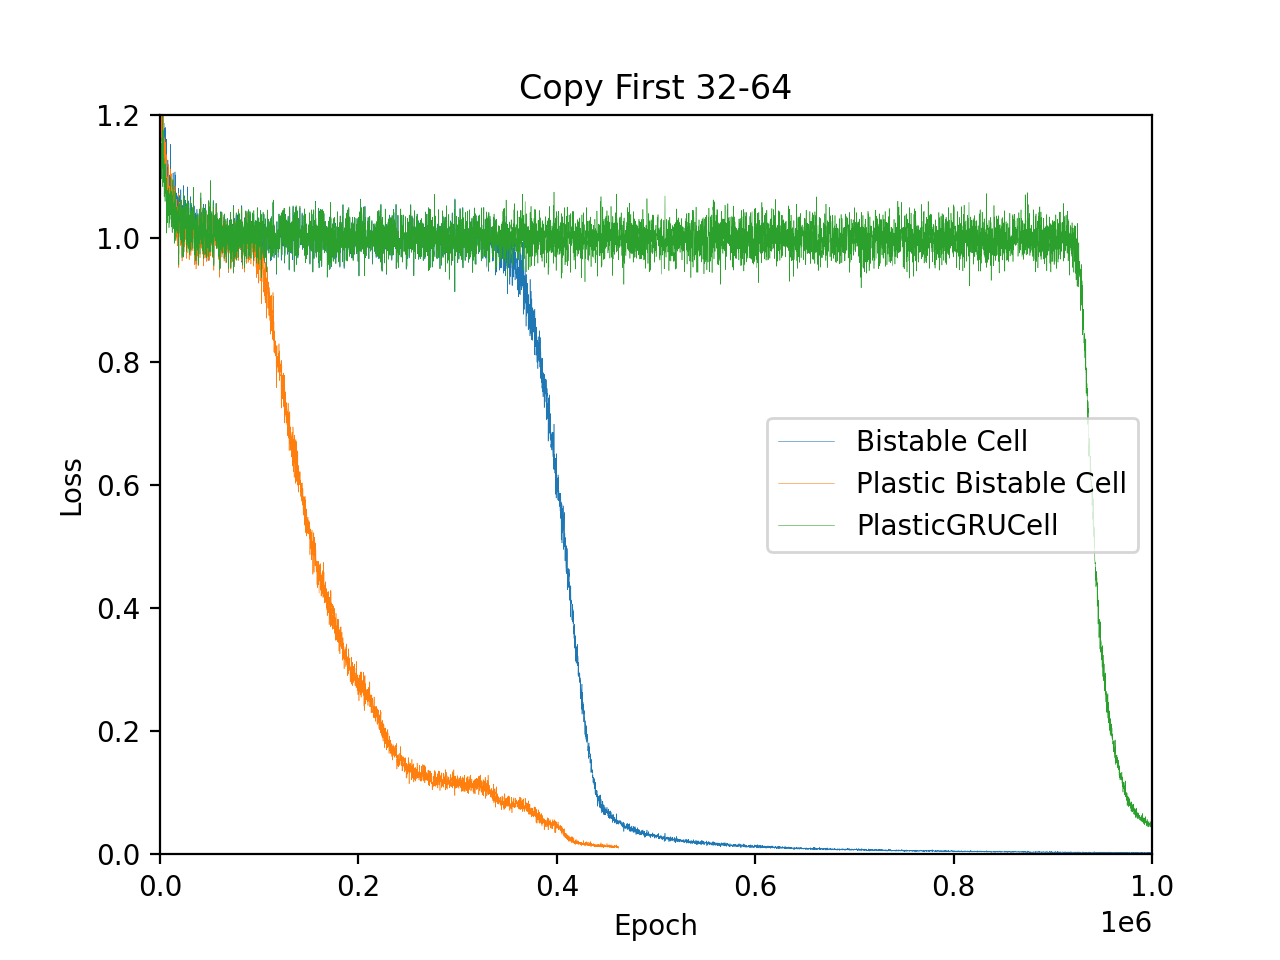
\includegraphics[width=5in]{plots/32_64_plot}
\end{figure}

\clearpage
Below are plotted the losses of the nBRC and PBRC during learning the copy first task with an input dimension of 32 and a hidden state dimension of 48. The curves are much more similar than the previous plots, indicating that the differences in their architecture are not as important when they are pushed to the limits of their memory capacity. The PBRC does solve the task usually roughly a quarter less data than the nBRC.
\begin{figure}[h]
	\centering
	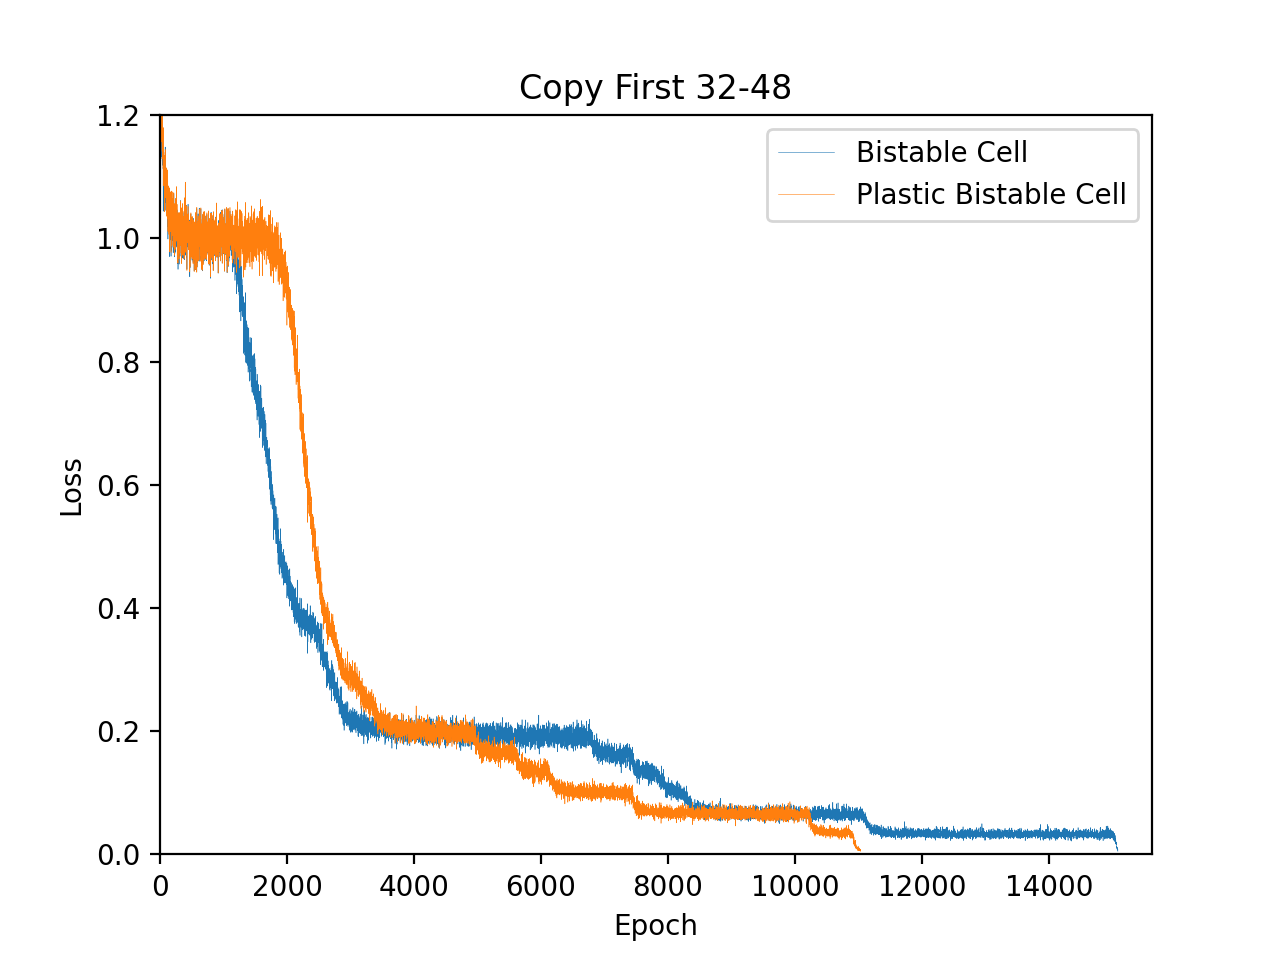
\includegraphics[width=5in]{plots/32_48_plot}
\end{figure}